\documentclass{report}
\usepackage{amsmath}
\usepackage{amssymb}
\usepackage{hyperref}
\usepackage{graphicx}
\usepackage{float}
\usepackage{listings}
\begin{document}
\section{LinearRegression without regularization}
\subsection{Abstract}
Hello, everyone. I'm btobab.\\
When I learned NLP, I found I completely can't understand formula derivation, so I decided to learn the theoretical derivation of machine learning from the beginning.\\
This chapter is mainly divided into two parts:
\begin{itemize}
	\item[] The first part will derive the closed-form solution of the linear regression(least squares method) from three perspectives of matrix, geometry, probability, and provide reference code.
	\item[] The second part will derive the closed-formula solution of least squares method with regularization from two perspectives of matrix and probability, and construct a complete linear regressioin class, and implement the closed-solution method and gradient descent method with code at the same time.
\end{itemize}
\subsection{Introduction}
Linear regression model is a model that use linear function to fit the relationship between one or more independent variables and the dependent variable ($y$).\\\\
The target variable ($y$) is a continuous numerical type, such as: housing price, number of people and rainfall. The regression model is to find a mapping function between input variables and output variables.\\\\
The learning of regression task equals to function fitting: use a function curve to make it fit the known data well and predict unknown data.\\\\
Regression task is divided into two processes: model learning and prediction. Construct a model based on given training dataset and predict corresponding output based on new input data.
\subsection{Algorithm}
\subsubsection{Matrix perspective}
Note:in general, the vectors we are discussing are column vectors. Therefore, in order to ensure the shape of the matrix during the derivation process, a large number of transposition characters are used\\\\
given dataset $\mathcal{D}=\{(x_1,y_1),(x_2,y_2)...(x_n, y_n)\}$\\\\
in which $x_i\in \mathcal{R}^p, y_i\in \mathcal{R}, i=1,2,...,n$

$$
X=(x_1,x_2,...,x_n)^T=\begin{pmatrix}
x_{11}&x_{12}&...&X_{1p}\\
x_{21}&x_{22}&...&x_{2p}\\
.&.&.&.&\\
.&.&.&.&\\
.&.&.&.&\\
x_{n1}&x_{n2}&...&x_{np}\\
\end{pmatrix}_{np}
$$
$$
Y=(y1,y2,...,y_n)_{n1}^T
$$
It is the model we constrct: $f(w)=w^Tx+w_0 x_0.$\\\\
Generally set $x_0=1$,and $b=w_0 x_0$, $b$ is bias, $w$ is weight. below, for the convenience of derivation, we merge $w_0$ into $w$ and $x_0$ into $x$.\\\\
so the model is updated to $f(w)=w^Tx$
The loss function of least squares method is:
$$
L(w)=\sum_{i=1}^{i=n}\|y_i-w^T x_i\|_2^2
$$
$$
=\begin{pmatrix}
y_1-w^Tx_1&y_2-w^Tx_2&...&y_n-w^Tx_n
\end{pmatrix}
\begin{pmatrix}
y_1-w^Tx_1\\
y_2-w^Tx_2\\
.\\
.\\
.\\
y_n-w^Tx_n\\
\end{pmatrix}
$$
$$
=(Y^T-w^TX^T)(Y^T-w^TX^T)^T
$$
$$
=(Y^T-w^TX^T)(Y-Xw)
$$
$$
=Y^TY-w^TX^TY-Y^TXw+w^TX^TXw
$$
Note the second and third terms are transposed to each other, and observe its matrix shape: $(1,p)(p,n)(n,1)=(1,1)$\\
Knowning that these two terms are scalars, and the transposition of a scalar is itself, so the two can be conbined, get:
$$
L(w)=Y^TY-2w^TX^TY+w^TX^TXw
$$
so $\hat{w}=argmin(L(w))$
below, to find out the minimum of $L(w)$, we need to diffentiate $L(w)$\\\\
Note there are three terms in the formual. The first term has nothing to do with $w$ and can be removed. Then the remaining two terms involve matrix derivation.\\\\
Regarding to matrix derivation, author recommends three articles by a blogger(more detailed and rigorous than textbook, each formual has proof)
\begin{itemize}
	\item \href{https://zhuanlan.zhihu.com/p/263777564}{essence}
	\item \href{https://zhuanlan.zhihu.com/p/273729929}{basics}
	\item \href{https://zhuanlan.zhihu.com/p/288541909}{advanced}
\end{itemize}
The following is the derivative solution process of the above two terms.\\\\
Because $X,Y$ are constant matrices, the derivative can be obtained directly. However, since it is the derivative of $w$, the result must be transposed.
$$
\frac{d(2w^TX^TY)}{dw}=2X^TY
$$
Below, let's solve the third term.
$$
d(w^TX^TXw)=tr(d(w^TX^TXw))=tr(X^TXd(w^Tw))
$$
$$
=tr(X^TX(d(w^T)w+w^Td(w)))=tr(X^TXw(dw)^T)+tr(X^TXw^Tdw)
$$
$$
=tr(w^TX^TXdw)+tr(X^TXw^Tdw)=tr(2X^TXw^Tdw)
$$
so

$$
\frac{d(w^TX^TXw)}{dw}=2wX^TX
$$
From a geometric perspective, we regard $X$ as a $p$ dimensional vector.\\\\
The first dimension of $X$ is $(x_{11},x_{21},...,x_{n1})$, the p-th dimension of $X$ is $(x_{1p},x_{2p},...,x_{np})$\\\\
and here $Y$ is regarded as a one-dimensional vector.\\\\
so $\frac{dL(w)}{dw}=2X^TXw-2X^TY$\\\\
set the derivative equal to 0 to get the closed-form solution of the least squares method:
$$
\hat{w}=(X^TX)^{-1}X^TY
$$
\subsubsection{Geometry perspective}
$$
X=(x_1,x_2,...,x_n)^T=\begin{pmatrix}
x_{11}&x_{12}&...&X_{1p}\\
x_{21}&x_{22}&...&x_{2p}\\
.&.&.&.&\\
.&.&.&.&\\
.&.&.&.&\\
x_{n1}&x_{n2}&...&x_{np}\\
\end{pmatrix}_{np}
$$
$$
Y=(y1,y2,...,y_n)_{n1}^T
$$
Now we assume  $p=2$ because it is easier to draw. The diagram is as follows(I really drew it for a long time and pitifully asked for a star.
\begin{figure}
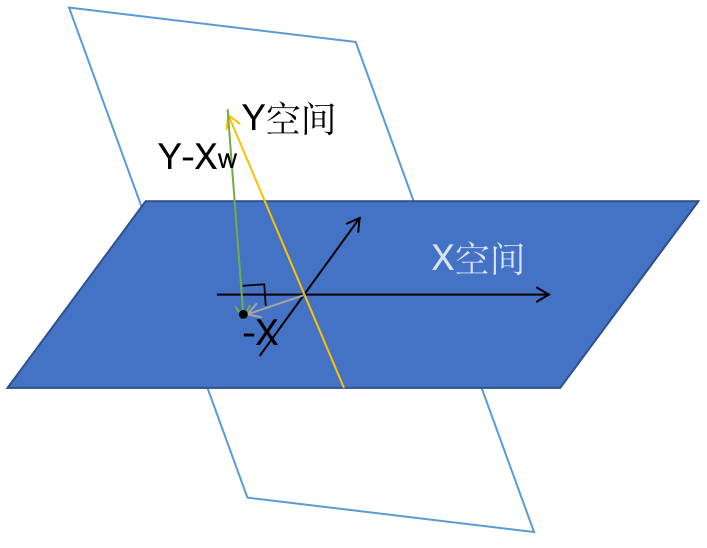
\includegraphics[width=0.7 \textwidth]{/Users/btobab/TeX-Projects/figures/1}
\caption{figure 1}
\end{figure}
Change the model to $f(w)=Xw$, which means zoom $X$ with weight $w$\\\\
The geometric meaning of the least squares method is to find a $w$, so that the distance between vector $Y-Xw$ and space $w$ is the smallest. Of course the case of the smallest distance is perpendicular to space $X$.\\\\
so we get a formula: $X^T(Y-Xw)=0$\\\\
then get the solution of $w$: 
$$
X^TXw=X^TY
$$
$$
\hat{w}=(X^TX)^{-1}X^TY
$$
we can see that the solved $w$ is the same as the result of matrix perspective.
\subsubsection{Probability perspective}
As we known, in reality, it is hard to fit a distribution with a straight line. True data must have some randomness, that is, noise.\\\\
so we assume noise $\epsilon\backsim N(0,\sigma^2)$\\
so $y=f(w)+\epsilon=w^Tx+\epsilon$\\
so $y|x;w\backsim N(w^Tx,\sigma^2)$\\
Bring it into the probability density function of gaussian distribution:
$$
p(y|x;w)=\frac{1}{\sqrt{2\pi}\sigma}e^{-\frac{(y-w^Tx)^2}{2\sigma^2}}
$$
Then use $MLE$ (maximum likelihood estimate)\\\\
Note: so-called MLE is to get the relative frequency via a large number of samples to approximate probability\\\\
Let's assume a function: $\zeta(w)=\log{p(Y|X;w)}$

Since $n$ data are independent, we can change the probability to a form of continuous mutiplication:

$\zeta(w)=\log{\Pi_{i=1}^np(y_i|x_i;w)}=\Sigma_{i=1}^n \log{p(y_i|x_i;w)}$

bring the probability density function of gaussian distribution into the formula:

$\zeta(w)=\Sigma_{i=1}^n(\log{\frac{1}{\sqrt{2\pi}\sigma}}-\frac{(y-w^Tx)^2}{2\sigma^2})$

since the former term has nothing to do with $w$, it can be ignored.

so:
$$
\hat{w}=argmax{\zeta(w)}
$$
$$
=argmax{ \Sigma_{i=1}^n -\frac{(y-w^Tx)^2}{2\sigma^2}}
$$
$$
=argmin{ \Sigma_{i=1}^n (y-w^Tx)^2}
$$
The conclusion obtained by using maximum likelihood estimation is the definition of least squares method.\\\\
This also shows that least squares method hides a assumption that noise is gaussian distribution.
\subsection{Implement}
\begin{lstlisting}[language={python}]
%matplotlib inline
import numpy as np
import matplotlib.pyplot as plt

# num of samples
n = 1000
# noise
epsilon = 1
X = np.expand_dims(np.linspace(0,100,1000), axis=-1)
w = np.asarray([5.2])
Y = X  w
# apply noise to X
X += np.random.normal(scale=epsilon, size=(X.shape))
X_T = X.transpose()
w_hat = np.matmul(np.linalg.pinv((np.matmul(X_T, X))), np.matmul(X_T, Y))
print(w_hat)
plt.scatter(X, Y, s=3, c="y")
Y_hat = X  w_hat
plt.plot(X, Y_hat)
plt.show()
\end{lstlisting}
\newpage
\section{LinearRegression with regularization}
\subsection{Algorithm}
\subsubsection{Matrix perspective}
Firstly, given a new loss functioin with regularization:
$$
\zeta(w)=\Sigma_{i=1}^{n}||y_i-w^T  x_i||^2 + \lambda  ||w||^2
$$
then the derivation of loss function from matrix perspective without regularization is referenced:
$$
\zeta(w)=Y^TY-2w^TX^TY+w^TX^TX w+\lambda  ||w||^2
$$
so$\hat{w}=argmax(\zeta(w))$\\\\
differentiate $\zeta(w)$:
$$
\frac{\partial \zeta(w)}{\partial w}=2X^TXw-2X^T Y+2\lambda  w 
$$
set the derivative equal to 0 to get the closed-form solution of least squares method with regularization:
$$
\hat{w}=(X^TX+\lambda  I)^{-1} X^TY
$$
$I$ is identity matrix
\subsubsection{Probability perspective}
assume noise $\epsilon \backsim N(0,\sigma_1^2) \ w \backsim N(0,\sigma_2^2)$

since $y=w^T x + \epsilon$

we get $y|w \backsim N(w^T x,\sigma_1^2)$
\\Next we use MAP(Maximum a posteriori estimate):

according to Bayes theorem:
$$
P(w|Y)=\frac{P(Y|w) P(w)}{P(Y)}
$$
$P(w)$ is a priori probability, $P(Y|w)$ is a likelihood probability, $P(Y)$ is normalized probability, priori probability is mutiplied by the likelihood probability and normalized to obtain the posteriori probability $P(w|Y)$.
actually $P(Y)$ is constant, so:
$$
\hat{w}=argmax(P(w|Y))=argmax(P(Y|w) P(w))=argmax(log(P(Y|w) P(w)))
$$
since samples are independent, we can change the probability to a form of continuous mutipication.
$$
=argmax(log(\prod_{i=1}^n P(y_i|w) P(w)))=argmax(\sum_{i=1}^n log(P(y_i|w)+ log(P(w))))
$$
bring it into probability density function of gaussian distribution to get:
$$
\hat{w}=argmax(\sum_{i=1}^nlog(\frac{1}{\sqrt{2\pi} \sigma_1})-\frac{(y_i-w^T x_i)^2}{2\sigma_1^2}+log(\frac{1}{\sqrt{2 \pi} \sigma_2})-\frac{w^2}{2\sigma_2^2})
$$
since both $\sigma_1$ and $\sigma_2$ are hyperparameters, they can be omitted.

so:
$$
\hat{w}=argmin(\sum_{i=1}^n \frac{(y_i-w^T x_i)^2}{2\sigma_1^2}+\frac{w^2}{2\sigma_2^2})
$$
$$
=argmin(\sum_{i=1}^n (y_i-w^T x_i)^2+\frac{\sigma_1^2}{\sigma_2^2} w^2)
$$
we can see that the result derived via $MAP$ is the definition of the least squares method with regularization.
\subsection{Implement}
\begin{lstlisting}[language={python}]
import os
os.chdir("../")
from models.linear_models import LinearRegression
import numpy as np
import matplotlib.pyplot as plt
X_ = np.expand_dims(np.linspace(0, 10, 1000), axis=-1)
X = np.c_[X_, np.ones(1000)]
w = np.asarray([5.2, 1])
Y = X.dot(w)
X = np.r_[X, np.asarray([[11, 1], [12, 1], [13, 1]])]
Y = np.r_[Y, np.asarray([100, 110, 120])]

model = LinearRegression(l2_ratio=1e1, epoch_num=1000, lr=1e-2, batch_size=100, if_standard=False)
model.fit(X[:, :-1], Y)
print(model.get_params())
model.draw(X[:, :-1], Y)
\end{lstlisting}
\end{document}